\scanpage{65}
\mspage{64}
% E: text|top left|3.1.84
3.1.84
% E: drawing|upper left|Delta_D' D' a a' s
\figure{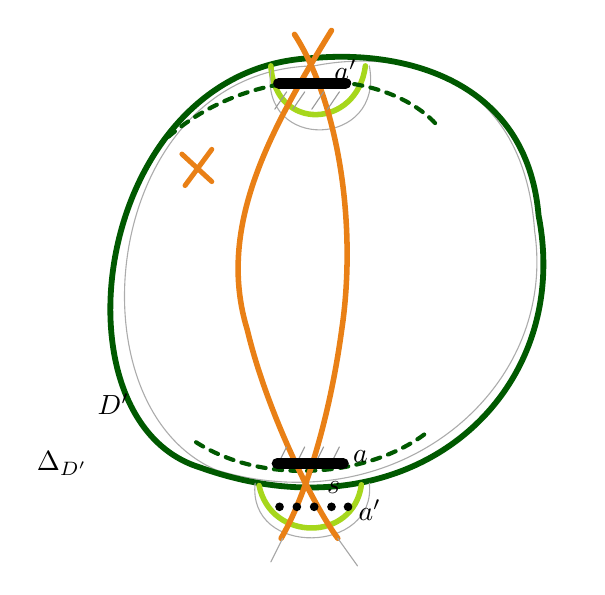
\begin{tikzpicture}[x=1cm,y=1cm,line cap=round,line join=round]
\draw[gray!65] (0,2.7) .. controls (-2.7,2.65) and (-3.15,-1.6) .. (-1.25,-2.43) .. controls (1,-3.12) and (3.1,-1.45) .. (2.8,.6) .. controls (2.65,2.7) and (1,2.9) .. (0,2.7);
\draw[green!35!black,line width=2.1pt] (0,2.8) .. controls (-2.8,2.7) and (-3.4,-1.8) .. (-1.45,-2.4) .. controls (1.2,-3.35) and (3.3,-1.5) .. (2.85,.8) .. controls (2.7,2.55) and (1.1,2.9) .. (0,2.8);
\draw[yellow!65!green,line width=2pt] (-.55,2.7) .. controls (-.5,1.85) and (.55,1.9) .. (.65,2.7);
\draw[gray!65] (-.55,2.65) .. controls (-.7,1.6) and (.9,1.65) .. (.7,2.7);
\draw[green!35!black,line width=1.5pt,dashed] (-1.85,1.8) .. controls (-.7,2.8) and (1,2.65) .. (1.6,1.9);
\draw[green!35!black,line width=1.5pt,dashed] (-1.5,-2.08) .. controls (-.6,-2.65) and (.7,-2.5) .. (1.4,-1.98);
\draw[yellow!65!green,line width=2pt] (-.7,-2.63) .. controls (-.55,-3.35) and (.5,-3.35) .. (.6,-2.62);
\draw[gray!65] (-.75,-2.6) .. controls (-.85,-3.55) and (.8,-3.5) .. (.7,-2.6);
\draw[orange!65!brown,line width=2pt] (-.25,3.1) .. controls (.3,2.25) and (.55,.7) .. (.35,-.65) .. controls (.2,-1.75) and (-.1,-2.75) .. (-.42,-3.3);
\draw[orange!65!brown,line width=2pt] (.22,3.15) .. controls (-.55,1.9) and (-1.25,.65) .. (-.85,-.65) .. controls (-.6,-1.7) and (0,-2.9) .. (.3,-3.3);
\draw[gray!70] (-.4,-3.3)--(-.55,-3.6) (.3,-3.3)--(.55,-3.65);
\foreach \x in {-.35,-.12,.12,.32}{\draw[gray!80] (\x,2.37)--(\x-.15,2.15);\draw[gray!80] (\x,-2.14)--(\x-.12,-2.38);}
\draw[line width=4pt] (-.45,2.48)--(.4,2.48);
\draw[line width=4pt] (-.47,-2.35)--(.37,-2.35);
\foreach \x in {-.44,-.22,0,.22,.43}{\fill (\x,-2.9) circle (.055);}
\draw[orange!65!brown,line width=1.8pt] (-1.68,1.58)--(-1.3,1.23) (-1.64,1.18)--(-1.3,1.64);
\node at (.4,2.65) {$a'$};\node[right] at (.37,-2.26) {$a$};\node[right] at (.44,-2.94) {$a'$};\node[right] at (.04,-2.65) {$s$};\node at (-2.55,-1.6) {$D'$};\node at (-3.2,-2.35) {$\Delta_{D'}$};
\end{tikzpicture}}
% E: drawing|upper middle|Delta_D D b b' s
\figure{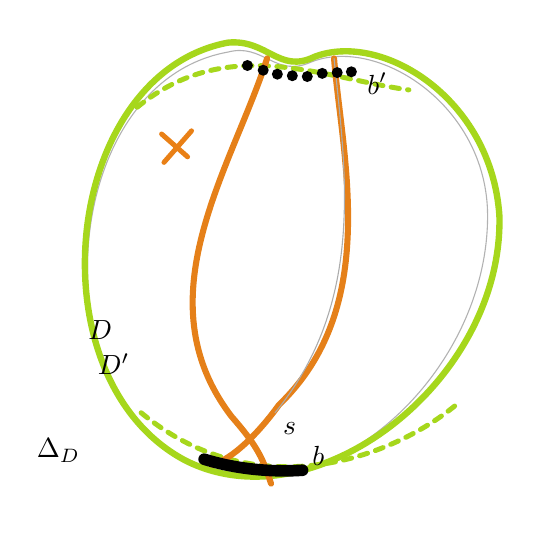
\begin{tikzpicture}[x=1cm,y=1cm,line cap=round,line join=round]
\draw[gray!60] (-.7,2.68) .. controls (-2.8,2.3) and (-3.1,-1.5) .. (-1.3,-2.5) .. controls (.4,-3.4) and (2.6,-1.5) .. (2.6,.6) .. controls (2.6,2) and (1.2,2.9) .. (.35,2.55) .. controls (-.1,2.35) and (-.25,2.8) .. (-.7,2.68);
\draw[yellow!65!green,line width=2.3pt] (-.7,2.8) .. controls (-2.8,2.4) and (-3.2,-1.45) .. (-1.25,-2.5) .. controls (.4,-3.35) and (2.8,-1.5) .. (2.75,.6) .. controls (2.65,2.1) and (1.25,2.95) .. (.4,2.62) .. controls (-.05,2.4) and (-.2,2.85) .. (-.7,2.8);
\draw[yellow!65!green,line width=1.8pt,dashed] (-1.85,1.98) .. controls (-.7,2.92) and (.5,2.35) .. (1.6,2.2);
\draw[yellow!65!green,line width=1.8pt,dashed] (-1.8,-1.9) .. controls (-.35,-3.1) and (1.35,-2.5) .. (2.2,-1.8);
\draw[orange!60!brown,line width=2.2pt] (-.2,2.6) .. controls (-.65,1.2) and (-1.8,-.45) .. (-.65,-1.95) .. controls (-.3,-2.35) and (-.25,-2.5) .. (-.15,-2.8);
\draw[orange!60!brown,line width=2.2pt] (.65,2.6) .. controls (.75,1.35) and (1.25,-.55) .. (-.05,-1.8) .. controls (-.3,-2.15) and (-.65,-2.5) .. (-.9,-2.56);
\draw[gray!65] (.65,2.6) .. controls (.8,1.15) and (1.05,-.5) .. (-.1,-1.9);
\foreach \x/\y in {-.45/2.51,-.25/2.45,-.07/2.4,.12/2.38,.31/2.37,.5/2.41,.69/2.42,.87/2.43}{\fill (\x,\y) circle (.07);}
\draw[line width=4.2pt] (-1,-2.49) .. controls (-.65,-2.6) and (-.2,-2.66) .. (.25,-2.63);
\draw[orange!65!brown,line width=1.8pt] (-1.54,1.64)--(-1.21,1.35) (-1.51,1.28)--(-1.16,1.68);
\node[right] at (.95,2.28) {$b'$};\node[right] at (.25,-2.45) {$b$};\node[right] at (-.12,-2.1) {$s$};\node at (-2.32,-.85) {$D$};\node at (-2.15,-1.28) {$\deleted{\unsure{D'}}$};\node at (-2.85,-2.38) {$\Delta_D$};
\end{tikzpicture}}
% E: text|below drawings across left two thirds|huit façons standart de recoller
huit façons ``standart'' de recoller $\Delta_D$ à $\Delta_{D'}$, \unsure{suiv\textsuperscript{t}} \deleted{\unsure{le}} \deleted{\unsure{une}} \unsure{isom.} choisi d'un des deux arcs de transition \inserted{$a,a'$} sur $\Delta_{D'}$, sur l'un des deux arcs privilégiés $b$ (de transition) et $b'$ (son antipodique) sur $\Delta_D$, deux choix pour chaque choix d'un couple dans $\{a,a'\}\times\{b,b'\}$. Donc huit façons à priori de construire une surface à bord \inserted{cellulaire} pour graphe $\Gamma_{\underline\Sigma}=\Gamma$, mais (sauf pour le \unsure{plongement} d'une courbe rouge, \unsure{différent}) il n'y a que quatre cas différents de surfaces, car \unsure{ceux} qu'on obtient pour un choix $(\alpha,\beta,\unsure{\rho|\sigma})$ \inserted{\unsure{iso. de recollement}} et $(\alpha',\beta',\sigma')$ (où $\alpha',\beta',\sigma'$ déduits en composant avec
% E: text|right column upper|les antipodismes
les antipodismes) sont can. isom. (ils correspondent à la $=$ circularisation de $\Gamma$, et les \unsure{$=$s|$=$} réflexions de transition pour les \unsure{or. loc.|syst. loc.} correspond. \unsure{du})

On peut \unsure{les supposer|donc supposer}, quitte à composer avec les antipodismes de part et d'autre, que $\beta=b$ --- ce qui revient à faire un choix où le sommet $s$ apparaît \deleted{\unsure{au}} au voisinage de l'arc de transition choisi, sur la surface recollée (au lieu qu'il soit rejeté aux antipodes, ce qui a l'air un peu idiot!)
% E: deletion|bottom right|P. cf les quatre dessins
\deleted{\unsure{P. cf} les quatre dessins (ou plutôt, les huit)} qui
